\documentclass[11pt]{article}

\usepackage[english]{babel}                 %% hyphenation rules, spell-checker
\usepackage{amsmath,amssymb}                        %% macros like align* and pmatrix
\usepackage{graphicx,epstopdf}              %% for .eps graphs
\usepackage[official]{eurosym}              %% 1 \euro
\usepackage[a4paper,margin=2cm]{geometry}   %% margins

\frenchspacing                              %% no extra space after period
\addtolength{\parskip}{0.5\baselineskip}    %% some white space between paragraphs
\setlength{\parindent}{0pt}                 %% but no indentation
\renewcommand{\baselinestretch}{1.1}        %% line spacing of TeX is small
\DeclareMathOperator{\E}{\mathbb{E}}

\title{Non-life --- Assignment NL1}  %% don't forget to change!

\author{
  Niels Keizer\footnote{Student number: 10910492}
  \quad and \quad
  Robert Jan Sopers\footnote{Student number: 99999999}
}

\date{\today}

\begin{document}

\maketitle

\section*{Generating multinormal and multi-student r.v.'s}

\subsection*{Q1}

First we run the following script:

\begin{verbatim}
> set.seed(1)
> sum(duplicated(runif(1e6))) ## = 120
[1] 120
> sum(duplicated(rnorm(1e8))) ## = 0
[1] 0
\end{verbatim}

The function \verb|duplicated| returns a logical array where unique numbers are marked with 0 and duplicates are marked with 1 (the first occurence of the number is marked with a 0). Summming this array thus gives the total number of duplicates. The uniform distribution gives 120 duplicates in a much smaller sample size than the normal distribution, which gives 0 duplicates.

In the assignment, the expected number of different numbers is derived to be 
\begin{displaymath}
  \E[N_n] = \frac{1 - f^n}{1-f}
\end{displaymath}

The number of duplicates is then given by 
$n - \E[N_n]$
We run the following script:

\begin{verbatim}
> m <- 2^32;n <- 1e6
> f <- 1 - 1/m
> num_dup_unif <- n - (1-f^n)/(1-f)
> num_dup_unif
[1] 116.3988
\end{verbatim}

The expected result of 116.4 is quite close to the generated result. The outcome of 120 is therefore consistent with the assumption that \verb|runif| produces different values uniformly.

The resolution of \verb|rnorm| is somewhere in the $2^50$'s. Directly calculating $1 - f^n$ will give $1$, because f is so close to $1$.
First, we use to approximation given in the assignment.
\begin{displaymath}
f^n = \left( 1 - \frac{1}{m}\right)^n \approx 1 - \frac{n}{m} + \frac{n^2}{2m^2}
\end{displaymath}

Inserting this into our equation for the number of different numbers gives
\begin{displaymath}
\frac{1 - f^n}{1-f} \approx \frac{1 - 1 + \frac{n}{m} - \frac{n^2}{2m^2}}{1- \left(1 - \frac{1}{m}\right)}  = \frac{\frac{n}{m} - \frac{n^2}{2m^2}}{\frac{1}{m}} = n - \frac{n^2}{2m}
\end{displaymath}

This results in the following equation for the expected number of duplicates.
\begin{displaymath}
n - \left(n - \frac{n^2}{2m}\right) = \frac{n^2}{2m}
\end{displaymath}

Next we check in \verb|R| if the number of duplicates is consistent with values for $m$ of $10^{15}$, $10^{16}$, $10^{17}$ or $10^{18}$, when $n$ is $10^8$
\begin{verbatim}
> n_norm <- 1e8
> m_norm <- c(1e15,1e16,1e17,1e18)
> num_dup_norm <- n_norm^2/(2*m_norm)
> num_dup_norm
[1] 5.000 0.500 0.050 0.005
\end{verbatim}

The obtained result seems to be consistent with a resolution of $10^{16}$ or higher.
 
\subsection*{Q2}
The following code is executed in \verb|R|.
\begin{verbatim}
> n <- 200; p <- 0.52
> x <- c(0,cumsum(2*rbinom(n,1,p)-1))
> plot(x, type="l", lwd=1, ylab="state", xlab="step", main="1-dimensional random walk")
\end{verbatim}
This gives the following biased random walk:

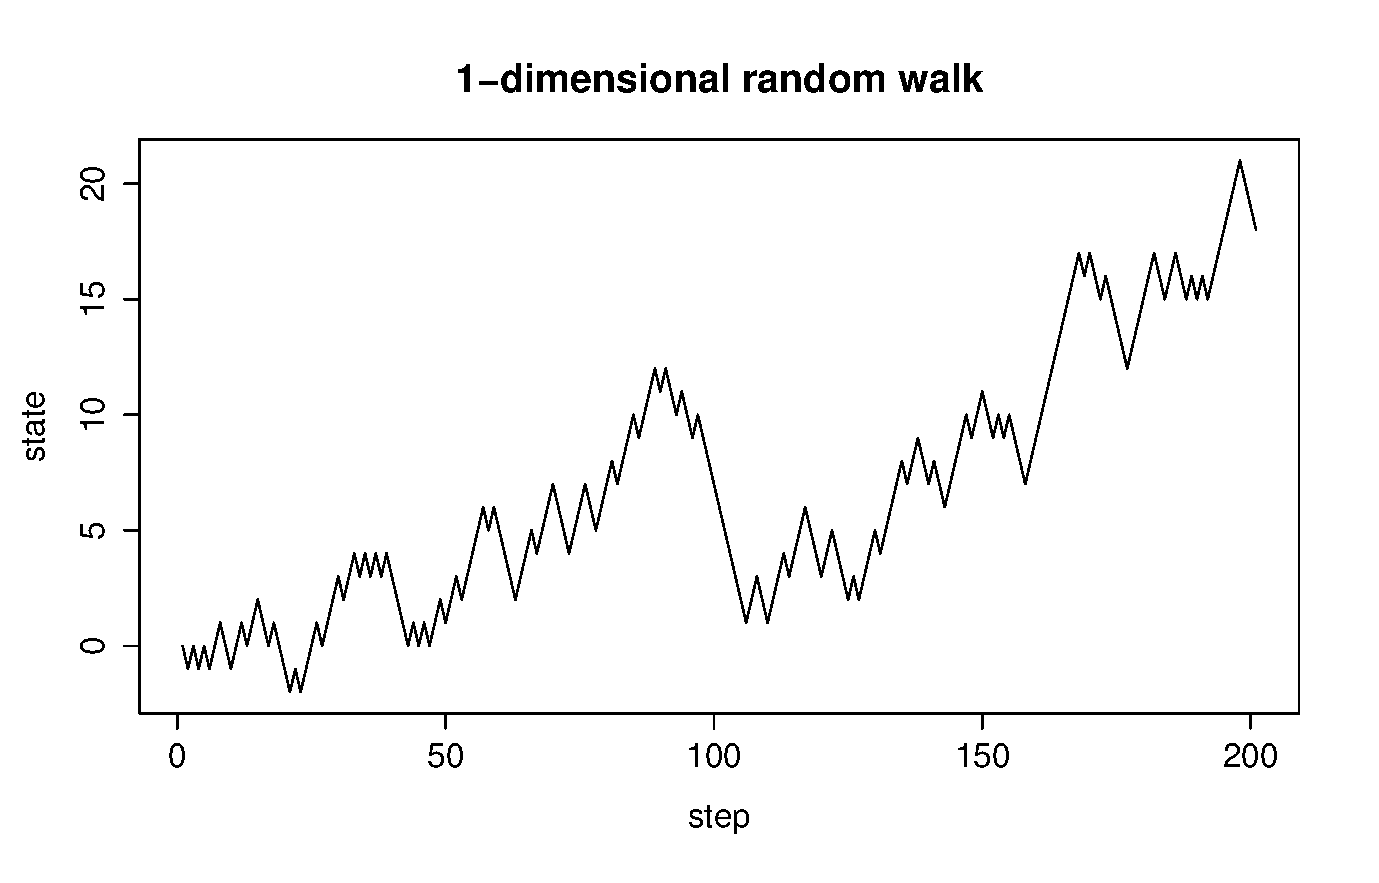
\includegraphics[scale=.6]{NL1_Q2_1D-randomwalk.eps} 


\end{document}
